\graphicspath{{./images/chap4/}}
% Relevance Feedback
% Methodology
% * Design and Architecture
% * Population of interest and sampling subject used in the study
% * Instrument and what it measures (metrics)
% * qualifications of informants if used in the study
% * Validation
% * Data gathering procedure (experiments)
\chapter{Relevance Feedback}
\label{chap:relevance_feedback}

To study and understand the effect of relevance feedback to the retrieval
results, we implement a simulator that reproduces the relevance feedback
processes of sloop. The implementation of the simulator is described in
\ref{sec:method} section. We then compare the initial ranked result set
outputted from SIFT computation with the results that undergo different rounds
of relevance feedback with various configurations in the \ref{sec:experiments}
section.

\section{Methodology}
\label{sec:method}

The relevance feedback simulator mimics the behavior of the task submission
process by the repeatedly sampling a batch of capture pairs from the pool of
all unknown capture pairs. For all the sampled pairs within a batch, the
simulator marks them as matching pairs or non-matching pairs with the
\emph{correct} answers.

When all the pairs in a specific batch are marked, it constructs an
\emph{identity graph} that represents the connections between all the known
pairs using the marked answers. The identity graph is undirected. The nodes in
the graph represent captures. If there is an edge connecting between node $A$
and $B$, capture $A$ and $B$ contain the same individual. Graphically mapping
the relationship of individuals results in fully-connected subgraphs formed by
all the captures containing the same animals.

Upon the retrieval of the new information from each batch, the simulator uses
the identity graph to infer the answers of the unknown pairs. This imitates the
in-database merging logic of the current version of Sloop\cite{sloopdocs}. The
transitive relations are drawn from both matching pairs and non-matching pairs.
For example, given capture $A$ is known to contain the same individual as that
in capture $B$, and capture $B$ is known to contain the same individual as that
in capture $C$, the simulator can infer that capture $A$ contains the same
individual as that in capture $C$, without having known the actual answer of
$A$ and $C$. Once such transitive inference is made, it adds $C$ to the
identity graph. Then, it continues to sample a new batch iteratively until the
distribution satisfies the convergence condition specified by the user.

The correctness of such inference relies on the validity of the premises, i.e.
if the answers to the matches are correct then the conclusion must also hold.
Problems arise when our seemingly \emph{correct} answers are, in fact,
incorrect. With the auto merging, the error propagates rapidly. An incorrect
answer yield erroneous results not only to the pair of captures in question,
but to \emph{all} the captures from the same cohorts as the captures in
question. However, incorrect answer can be  detected once inconsistency among
the answers emerges. In the actual Sloop production, all the captures within
the cohorts related to the captures in which inconsistency apears are going to
be send for expert manual review for reevaluation. On the other hand, in our
simulation, we would like to examine the consequences of the incorrect answers.
Therefore, the simulator also allows users to specify the error probability at
the initialization.

\section{Metrics} % (fold)
\label{sec:metrices}

This section describes the metrics used to evaluate the performance our
models. Along with our goal to maximize the precision and recall, we would like
to minimize the cost of the crowdsourced feedback or to operate optimally within a
budget constraint. The simulator also provides a counter that counts the number
of iterations a distribution takes to converge. However, this is out of our
interest because the time a model takes to converge can also be inferred from
the number of task submitted. Given a model, the fewer assignments posted, the
faster the model converges. 

\subsection{Precision and Recall} % (fold)
\label{sub:precision_and_recall}

As you can see, in the system where true negatives (true non-matching pairs)
largely outnumbers the true positives (true matching-pairs), comparing the
\emph{true positive rate (TPR)} or recall to the \emph{false positive rate
(FPR)} is not very meaningful. This is because false positive rate, which is
$\Pr{(\hat{y}=1|y=0)} = \frac{FP}{FP+TN}$, is going to be approximately 0 as
$TN$ is very large. Thus, instead of using ROC (receiver operating
characteristic) curve, which is a plot of TPR and FPR, we use
\emph{precision-recall curves (PR)} to analyze the performance of our models.

A precision recall curve is a plot of precision and recall as we  vary the
threshold $\theta$. Precision or positive predictive value (PPV) is defined as
following \cite{manning2008introduction}: $$PPV = \Pr{(y=1|\hat{y}=1)} =
\frac{TP}{\hat{P}} = \frac{TP}{TP+FP}$$

We evaluate the ranked retrieval performance of different relevance feedback
sampling policies using the \emph{Mean Average Precision (MAP)}, which is
roughly the area under the \emph{precision-recall curves}.
% subsection precision_and_recall (end)

\subsection{Cost} % (fold)
\label{sub:cost}

The total amount of money we have to spend to reward the workers is
proportional to the \emph{number of tasks we published}. If, at the moment we
have just finished marking all the unknown pairs, there are still some leftover
tasks on the crowdsourcing, those tasks are not going to be cancelled (unless
the user forcefully cancels the tasks himself.) Hence, we can use the number of
tasks we published as our cost metric.
% subsection cost (end)

% section metrics (end)

\section{Experiments} % (fold)
\label{sec:experiments}

In this section, we consider a setting in which time evolves in rounds. In each
round, the we, the requester, simulates the task submission process in a
crowdsourcing platform assuming that all the workers completes all the task.
Our goal as the requester is to maximize the Mean Average Precision value of a
preliminary score distribution outputted from Sloop with the amount payments we
have to make in mind.

We report three experiments corroborating the improvement of the retrieval
results after various rounds of relevance feedback and different sampling
strategies.  Experiment \ref{sub:batch_sizes} establishes that relevance
feedback improves the accretion of precision and recall of the preliminary
results at various batch sizes.  Experiment \ref{sub:errors} shows the
consequence of the erroneous answers at different error probabilities.
Experiment \ref{sub:sampling_policies} compare the performance of various
sampling policies.

All experiments are performed on the Grand and Otago dataset described in
Chapter \ref{cha:datasets}. Both datasets are annotated by the biologist, which
we take as our true labels. Table 

\begin{table}[t]
\captionsetup{justification=centering}
  \caption{Number of capture pairs for each species}
  \label{species-num-pairs} %chktex 24
  \centering
  \begin{tabular}{lc}
    \toprule
    Species & Number of pairs \\
    \midrule
    Grand & 507528 \\
    Otago & 492690 \\
    \bottomrule
  \end{tabular}
\end{table}

\subsection{Batch Sizes} % (fold)
\label{sub:batch_sizes}

This experiment first shows that relevance feedback improves the accretion of
precision and recall of the preliminary results at different iterations and
batch sizes. To establish these relations, we randomly sample some unknown
pairs from our unknown pair pool using \emph{uniform} sampling policy, in which
drawing each unknown pair is equally probable. The reason we use uniform random
sampling policy is because it is simple and unbiased, which is useful to get a
general baseline value.

During the sampling process, we observe the Mean Average Precision (MAP) at
each iteration. A batch of samples is iteratively drawn until we know the
answers to \emph{all} the unknown pairs or MAP is equal to 1, whichever happens
first.

We then repeat the process for various batch sizes, which is defined to be the
total number of unknown pairs marked in between a pair of the following events:
initialization, identity inference, and termination. Finally, we compare the
number of pairs sampled to reach convergence for each batch size.
% subsection batch_sizes (end)

\subsection{Errors} % (fold)
\label{sub:errors}

Despite the tasks distribution and the gold standard questions, there is
probability of 0.078 of obtaining an incorrect answer, assuming that all the
preventive events are independent. However, in practice, errors occur
haphazardly rather than systematically. Thus, 0.078 is the worst case, where we
assumed the worker always make a guess with equal probability.

This experiment models such error. Given an error probability of $\epsilon$, if
a pair of captures is sampled, the simulator marks it with the annotated answer
(correct answer) with the probability of $1-\epsilon$; otherwise, the pair is
marked with the opposite label (incorrect answer). Again, we compare the values
of MAP at each iteration and the total number of pairs sampled for each error
probability.
% subsection errors (end)

\subsection{Sampling Policies} % (fold)
\label{sub:sampling_policies}

Sampling policy plays a significant role in the retrieval. Given an initial
ranking, a pair of captures whose score is within a certain range or higher
than certain threshold is more likely to be a match. Such range and threshold
is species-specific and relies on Sloop's classification performance.

We experiment with following policies:
\begin{description}
  \item [Uniform]
  Sample an unknown pair from a uniform distribution where drawing each
    \emph{pair} is equally probable.
  \item [UniformScore]
  Sample an unknown pair from a uniform score distribution where drawing a pair
    with each \emph{score} is equally probable.
  \item [TopMatches]
  Always select an unknown pair with the highest score.
  \item [Nonmatches]
  Always select an unknown pair with the lowest score.
  \item [Normal]
  Sample an unknown pair from a normal distribution with $\mu=$median and
    $\sigma=0.3$.
  \item [Percentile]
  Always select an unknown pair at the median.
  \item [AllScores]
  Divide the scores into $n$ bins, where $n=$\texttt{batch\_size} and then
  select some unknown pairs from all the bins so that the total number of
  unknown pairs sums to \texttt{batch\_size}.
\end{description}

% subsection sampling_policies (end)

% section experiments (end)

\section{Results and Discussion} % (fold)
\label{sec:results}

Figure \ref{pr_curves} displays the Precision-Recall graph at a given number of
sampled unknown pairs. With zero error probability, relevance feedback reduces
the number of comparisons required for each specifies by a factor of 317 and
307 for grand and otago respectively. Within four iterations of feedback loop,
Mean Average Precision (MAP) reaches 1.0.

The results corroborates the fact that the relevance feedback dramatically
accretes precision and recall given the correct feedback information. Such
inclination of precision and recall is expected largely due to the
interpolation of the new information.

\begin{figure}[h!]
  \centering
  \subfloat[Grand]{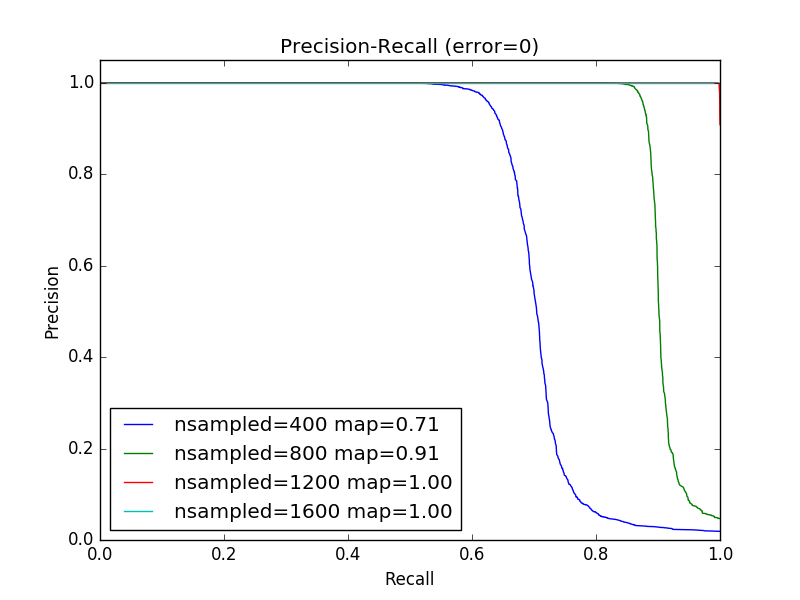
\includegraphics[width=0.8\textwidth]{pr/grand}}\\
  \subfloat[Otago]{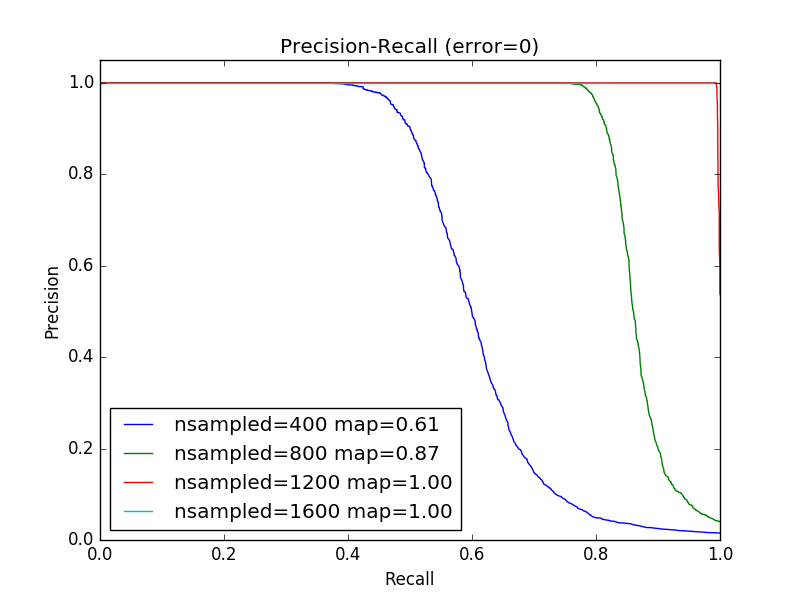
\includegraphics[width=0.8\textwidth]{pr/otago}}
  \captionsetup{justification=centering}
  \caption{Precision-Recall graph ($Error=0$, \texttt{batch\_size}$=400$)}
  \label{pr_curves}
\end{figure}

\subsection{Batch Sizes} % (fold)
\label{sub:batch_sizes_res}

Overall, from the graphs, MAP increases as we feed more data into the system.
Figure \ref{fig:sizes_curves} indicates that we publish more unnecessary
tasks as we increase the batch size. The fewer captures there are in a batch,
the lower the overall cost. Taking this idea one step further, we would like to
infer the matches and merge the individuals as frequently as possible. However,
empirically, smaller batch size may upset some workers who would like to
continuously work on the tasks. Therefore, we need to find the smallest batch
size that is still large enough to engage the workers.

\begin{figure}[h!]
  \centering
  \subfloat[Grand]{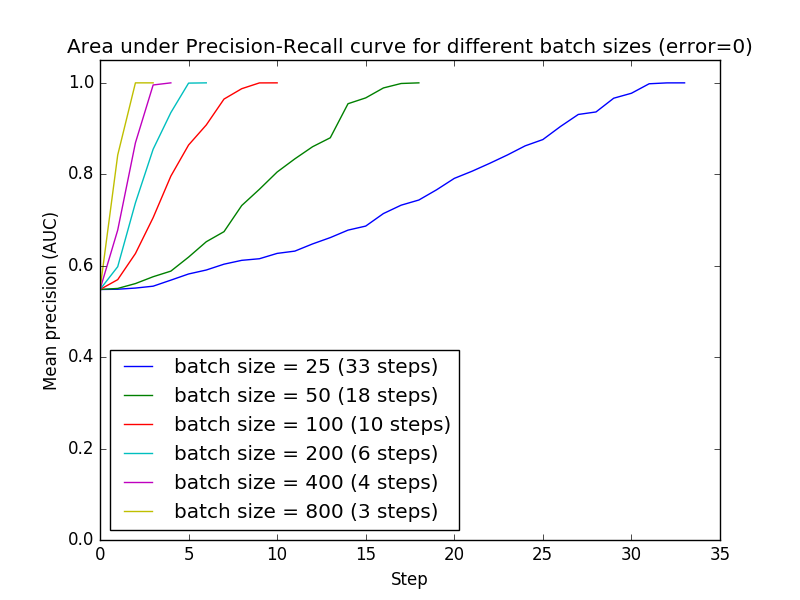
\includegraphics[width=0.8\textwidth]{sizes/graoc}}\\
  \subfloat[Otago]{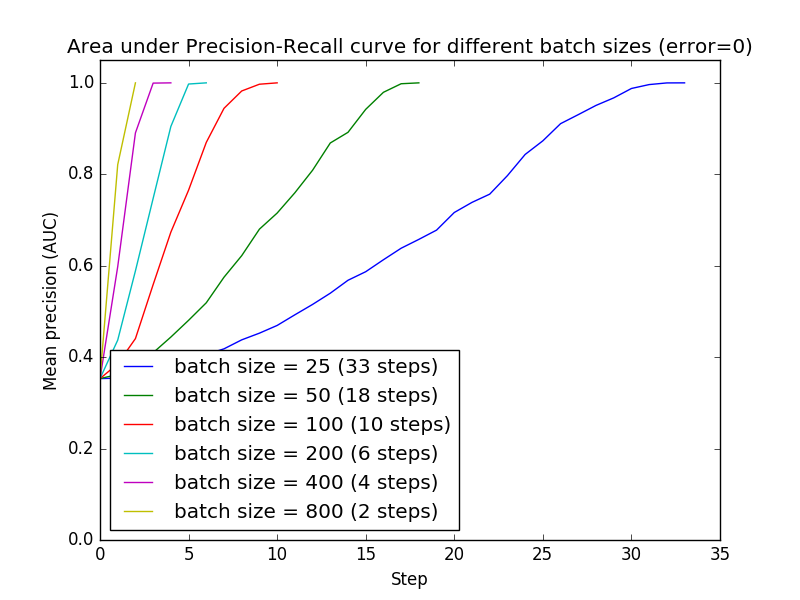
\includegraphics[width=0.8\textwidth]{sizes/otaoc}}
  \captionsetup{justification=centering}
  \caption{Mean Average Precision (MAP) for different batch sizes ($Error=0$)}
\end{figure}

\begin{figure}[h!]
  \centering
  \subfloat[Grand]{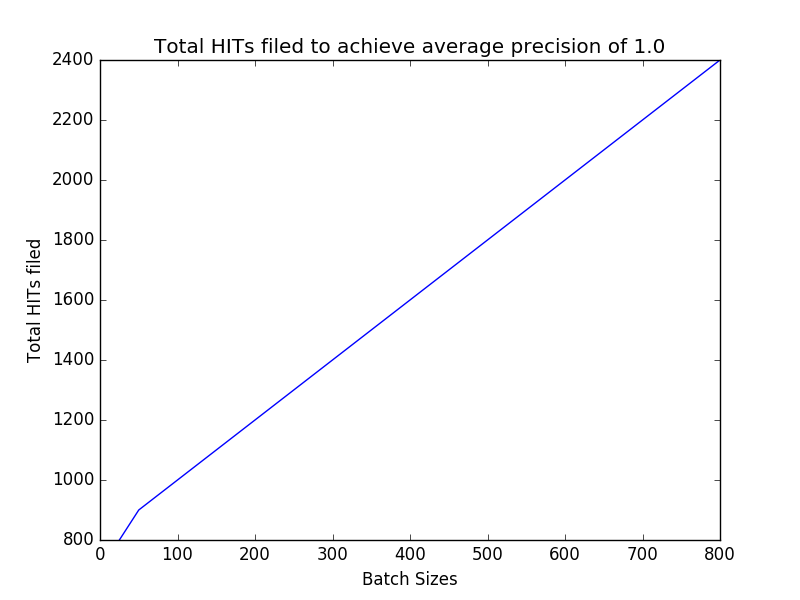
\includegraphics[width=0.8\textwidth]{sizes/grtotal}}\\
  \subfloat[Otago]{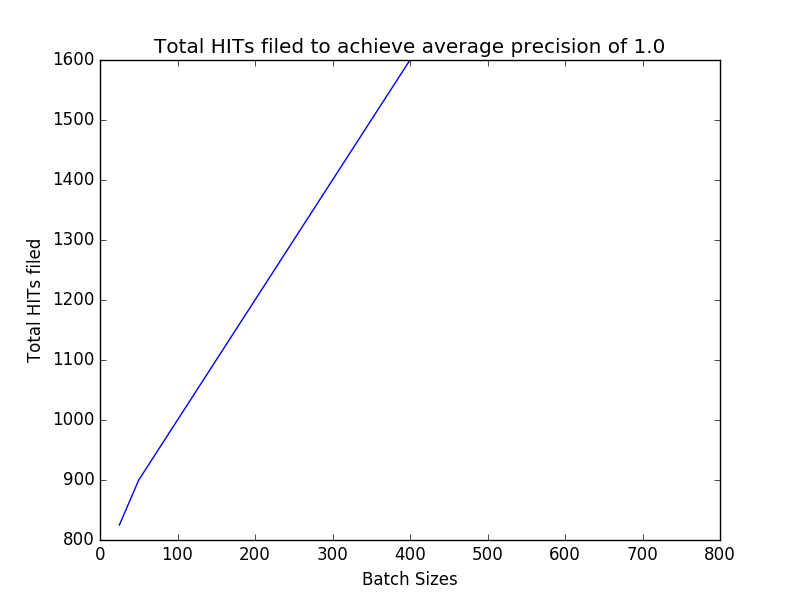
\includegraphics[width=0.8\textwidth]{sizes/ottotal}}
  \captionsetup{justification=centering}
  \caption{The total number of unknown pairs marked to achieve $MAP=1$
  ($Error=0$, \texttt{batch\_size}$=100$). Notice that this equals the total 
  number of tasks published to achieve $MAP=1$. }
  \label{fig:sizes_curves} %chktex 24
\end{figure}

% subsection batch_size (end)

\subsection{Errors} % (fold)
\label{sub:errors}

Despite the present of errors, relevance feedback still yields higher MAP
overall with an error threshold of 0.05. With a nonzero error probability, MAP
curves downward before it curves up and reach a saturation point. This is
because initially when it does not have much data, the system is very sensitive
to errors, especially the false negatives, which trigger the irreversible merge
operation. Thus, the precision decline rapidly.  As it gains more correct data,
it is able to recover from the downward phase. However, the historical merges
resulted from the past faulty data are irrevocable, so the precision saturates
eventually.

\begin{figure}[ht]
  \centering
  \subfloat[Grand]{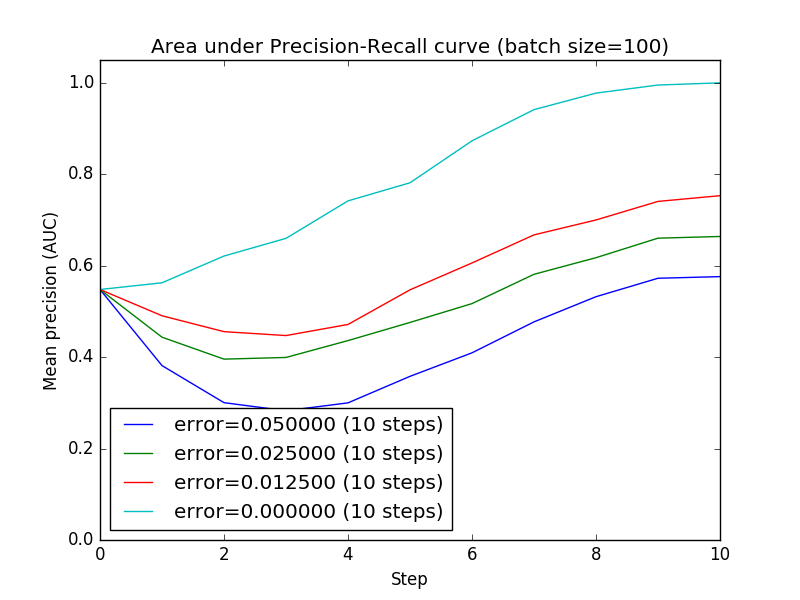
\includegraphics[width=\textwidth]{errors/graoc}}
  \caption{Mean Average Precision for different probabilities of error}
  \label{fig:grand_aoc} %chktex 24
\end{figure}
% subsection errors (end)

\subsection{Sampling Policies} % (fold)
\label{sub:sampling_policies_res}

Uniform sampling (Uniform), normal sampling (Normal), and sampling from all the
scores (AllScores) seem to outperform other sampling policies in term of the
total cost. The samplers that sample single score values at a time, such as
sampling from median (Percentile), performs poorly compare to others. However,
this depends largely on the species of the animal that we are interested in. As
you can see the performance of the each sampling policy differs slightly
between grand and otago.

\begin{figure}[h!]
  \centering
  \subfloat[Grand]{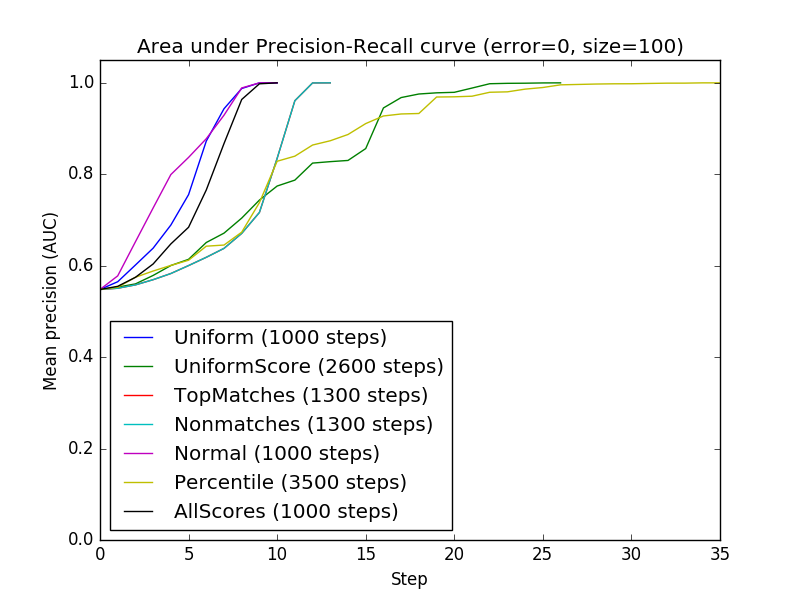
\includegraphics[width=0.8\textwidth]{policies/grand}}\\
  \subfloat[Otago]{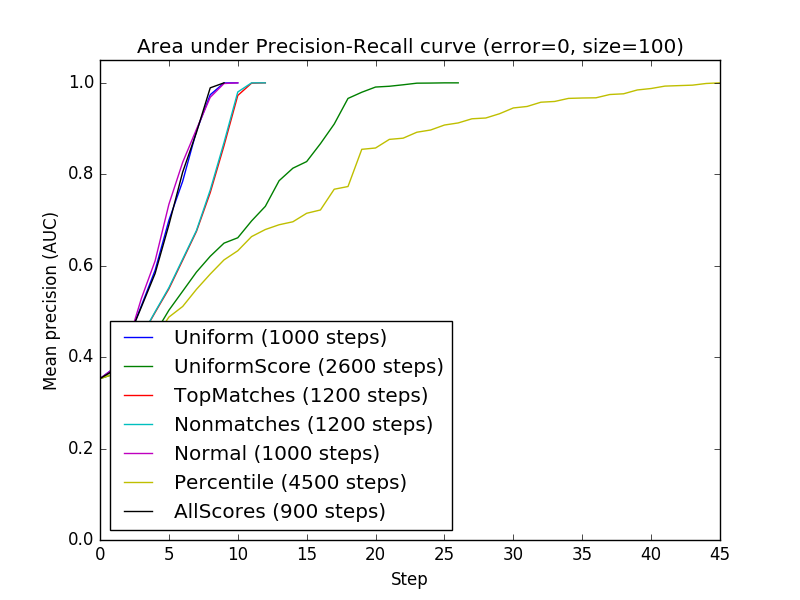
\includegraphics[width=0.8\textwidth]{policies/otago}}
  \captionsetup{justification=centering}
  \caption{Mean Average Precision (MAP) for various sampling policies ($Error=0$,
    \texttt{batch\_size}$=100$)}
\end{figure}
% subsection sampling_policies (end)

% section results (end)
